\section{Detailed Model, Contract, and Evaluation Tables}

\subsection{Running-scenario identifiers}

Table~\ref{tab:running-example} spells out the exact objects used for the
\path{refrigerated_counter1} scenario.  Display labels are shortened in the
prose, while execution uses these stable identifiers.

\begin{table*}[h]
  \caption{Exact contract objects for the Steinpilz
  \texttt{refrigerated\_counter1} interaction.}
  \label{tab:running-example}
  \small
  \begin{tabularx}{\textwidth}{@{}p{28mm}Y Y@{}}
    \toprule
    Element & Exact instance & Runtime meaning \\
    \midrule
    Target
      & \path{refrigerated_counter1} $\rightarrow$
        \path{ENT-ASSET-REFRIGERATED_COUNTER1}; group
        \path{ENT-GROUP-PRODUCT_COUNTERS}; zone
        \path{ENT-ZONE-PRODUCT_DISPLAY_ZONE}
      & Collider observation and trusted model referent \\
    Use case and scenario
      & \path{UC-STEINPILZ_BRAND_ROOM-INTERACT-REFRIGERATED_COUNTER1};
        \path{SC-STEINPILZ_BRAND_ROOM-INTERACT-REFRIGERATED_COUNTER1-MAIN}
      & User-facing interaction and executable flow \\
    Answer step
      & \path{STEP-STEINPILZ_BRAND_ROOM-INTERACT-REFRIGERATED_COUNTER1-ANSWER}
      & Scenario occurrence requiring one capability use \\
    Capability use
      & \path{CU-STEINPILZ_BRAND_ROOM-INTERACT-REFRIGERATED_COUNTER1-ANSWER-ROOM-GROUNDED-QUESTION};
        provider \path{ENT-AGENT-PRODUCT_SPECIALIST_AGENT}
      & Explicit target tuple and provider \\
    Capability
      & \path{CAP-STEINPILZ_BRAND_ROOM-ANSWER-ROOM-GROUNDED-QUESTION}
      & Operation declared for the Product Specialist Agent \\
    Binding and action
      & \path{RB-STEINPILZ_BRAND_ROOM-ANSWER-ROOM-GROUNDED-QUESTION};
        \path{RA-STEINPILZ_BRAND_ROOM-BACKEND-CHAT}
      & Exact realization at \texttt{POST /chat} \\
    Assertion and case
      & \path{SA-STEINPILZ_BRAND_ROOM-ANSWER-GROUNDED};
        \path{VC-STEINPILZ_BRAND_ROOM-INTERACT-REFRIGERATED_COUNTER1}
      & Declared identifier agreement and validation scope \\
    \bottomrule
  \end{tabularx}
\end{table*}
\FloatBarrier

\subsection{Runtime terminology}

Table~\ref{tab:runtime-terms} maps the shorter terms used in
Section~\ref{sec:implementation} to the exact repository and model
terminology.

\begin{table*}[h]
  \caption{Reader-facing runtime terms and their exact artifact counterparts.}
  \label{tab:runtime-terms}
  \small
  \begin{tabularx}{\textwidth}{@{}p{31mm}p{48mm}Y@{}}
    \toprule
    Paper term & Repository or model term & Meaning \\
    \midrule
    Room contract
      & FunctionalMLDS V2 instance;
        \path{functionalmlds.v2.instance.json}
      & Authoritative room-specific model containing interaction, execution,
        and evidence relations. \\
    Runtime map
      & Trace map and runtime context
      & Executable subset used by the client and backend to resolve one
        target-specific interaction path. \\
    Content hash
      & Model hash and contract fingerprint
      & Digest that binds the room contract, generated projections, and active
        session to the same model version. \\
    Situated capability
      & \texttt{CapabilityUse}
      & One occurrence that links a scenario step, target, provider, and
        reusable capability. \\
    \bottomrule
  \end{tabularx}
\end{table*}
\FloatBarrier

\subsection{FunctionalMLDS element and relation map}

Table~\ref{tab:functionalmlds-relations} complements the interaction-focused
view in Figure~\ref{fig:functionalmlds-core}.  It records the selected model
elements and references used to construct the complete
\contractpath{} paths evaluated in RQ1; it is a compact map rather than a full
serialization schema.

\begin{table*}[h]
  \caption{Selected FunctionalMLDS elements and relations underlying the
  runtime projection.}
  \label{tab:functionalmlds-relations}
  \small
  \begin{tabularx}{\textwidth}{@{}p{37mm}Y Y@{}}
    \toprule
    Elements & Key relation & Role in the running scenario \\
    \midrule
    \texttt{DynamicFunctionalModel}; \texttt{RequirementsModel};
    \texttt{UseCaseDefinitionSet} $\rightarrow$
    \texttt{UseCaseDefinition} $\rightarrow$ \texttt{UseCase}
      & One room-specific root links the selected UML/EAST-ADL requirements and
        use-case foundation to interaction, execution, and validation elements.
      & Fixes the authoritative cheese-booth model and scopes the visitor goal
        represented by the counter interaction. \\
    \texttt{UseCaseScenarioSpecification} $\rightarrow$
    \texttt{Scenario} $\rightarrow$ \texttt{ScenarioStep}
      & A use case is refined into ordered steps that identify the performer and
        the interaction occurrence.
      & Represents selection of \texttt{refrigerated\_counter1}, the question,
        and the grounded-answer step. \\
    \texttt{Actor}; \texttt{Entity};
    \texttt{Agent} $\subseteq$ \texttt{Entity}
      & Stable entity/source identifiers ground scene objects; agents additionally
        reference capabilities, asset/group/zone responsibilities, and permitted
        handoffs.
      & Identifies the counter, the active Reception Agent, and the responsible
        Product Specialist Agent. \\
    \texttt{CapabilityUse} $\rightarrow$ \texttt{Capability}
      & A situated capability use names its scenario step, provider, and targets
        and resolves one reusable capability.
      & Binds the Product Specialist Agent and selected counter to the
        grounded-answer capability. \\
    \texttt{RuntimePlatform}; \texttt{RuntimeBinding} $\rightarrow$
    \texttt{RuntimeAction}
      & The declared capability is realized by one platform-specific binding and
        concrete endpoint, tool, or event.
      & Resolves the accepted interaction to the exact backend-chat action rather
        than a generic chat dispatch. \\
    \texttt{Effect} $\rightarrow$ \texttt{Assertion}; runtime observation;
    \texttt{VerificationValidation}/\texttt{VVCase}
      & Assertions define expected results, observations record runtime evidence,
        and validation cases cover the relevant binding and assertions.
      & Requires returned target, provider, route, and action identifiers to agree
        before the answer is presented. \\
    \bottomrule
  \end{tabularx}
\end{table*}
\FloatBarrier

\subsection{Separate implementation capture}

Figure~\ref{fig:unity-binding-capture} records the exact
collider-to-entity binding used by the Unity client.  It depicts
\texttt{brand\_panel3}, because it is a frozen implementation capture rather
than the running cheese-counter walkthrough; both objects use the same exact
entity/source-ID mechanism.

\begin{figure}[h]
  \centering
  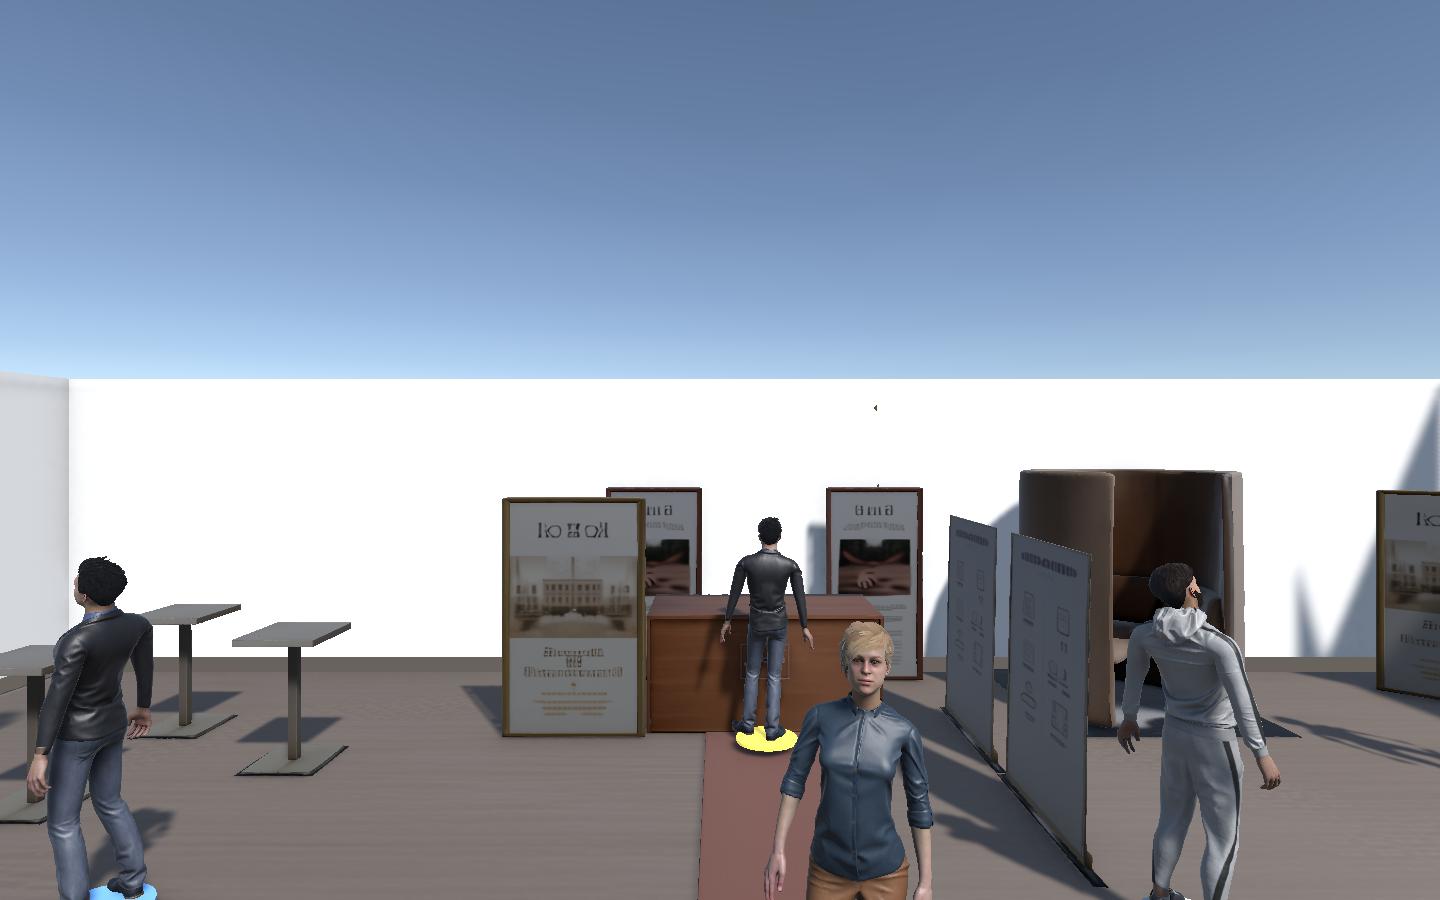
\includegraphics[
    alt={Unity Game view with a selected product panel and embodied agents},
    width=.82\columnwidth
  ]{../paper/figures/unity-model-grounded-selection.png}
  \caption{Separate Unity desktop implementation capture.  The selected
  \texttt{brand\_panel3} collider is bound to its stable model entity; the main
  text uses \texttt{refrigerated\_counter1} as the running scenario.}
  \Description{A Unity Game view of a virtual exhibition room with embodied
  agents and product panels.  One panel is highlighted and annotated with its
  stable source and model entity identifiers.}
  \label{fig:unity-binding-capture}
\end{figure}
\FloatBarrier

\subsection{Per-case structural results}

\begin{table}[h]
  \caption{Complete interaction paths. ``Pairs'' are asset-targeting
  \texttt{ScenarioStep}/\texttt{CapabilityUse} pairs.}
  \label{tab:per-case-chains}
  \small
  \begin{tabular}{@{}lrrrr@{}}
    \toprule
    Case & Assets & Complete & Pairs & Complete \\
    \midrule
    Career fair & 27 & 27 & 54 & 54 \\
    Classroom & 36 & 36 & 72 & 72 \\
    Brand room & 30 & 30 & 60 & 60 \\
    \midrule
    Total & 93 & 93 & 186 & 186 \\
    \bottomrule
  \end{tabular}
\end{table}

\begin{table*}[h]
  \caption{Offline structural routes from every modeled starting agent.
  ``Transitive'' and ``reachable'' are graph properties, not one-turn online
  execution.}
  \label{tab:per-case-routing}
  \small
  \begin{tabular}{@{}lrrrrrr@{}}
    \toprule
    Case & Probes & Local & Direct & Transitive & Unreachable & Reachable \\
    \midrule
    Career fair & 135 & 27 & 53 & 55 & 0 & 135 \\
    Classroom & 144 & 36 & 81 & 9 & 18 & 126 \\
    Brand room & 180 & 30 & 71 & 79 & 0 & 180 \\
    \midrule
    Total & 459 & 93 & 205 & 143 & 18 & 441 \\
    \bottomrule
  \end{tabular}
\end{table*}
\FloatBarrier
\clearpage

\subsection{Enforcement layers}

\begin{table*}[h]
  \caption{Representative invariants and failure boundaries in the implemented
  interaction path.}
  \label{tab:enforcement-layers}
  \small
  \begin{tabularx}{\textwidth}{@{}p{31mm}Y Y@{}}
    \toprule
    Layer & Representative invariant & Failure boundary \\
    \midrule
    JSON schema
      & Required fields, types, enumerations, reference shapes
      & Before constructing a model instance \\
    Canonical V2 model
      & Referential closure, typed cardinalities, source-ID uniqueness,
        assertion/validation ownership, no direct step-to-action shortcut
      & Instance rejected before materialization \\
    Executable profile
      & One provider and capability per occurrence, provider/performer/target
        agreement, complete binding and action
      & Invalid chains are not published \\
    Backend runtime
      & Pinned hash, unique trusted entity, derived group/zone, unique provider,
        local/direct route, exact target-specific action, request/response schema
      & Before generation and mutation when request-decidable; rollback after a
        response-dependent failure \\
    Unity client
      & Exact collider binding, explicit unresolved states, returned
        target/provider/route/action agreement
      & Before request serialization or answer presentation; backend remains
        authoritative \\
    \bottomrule
  \end{tabularx}
\end{table*}
\FloatBarrier

\section{Artifact Map}

The reproducible benchmark is rooted at
\texttt{research/iui2027/evaluation}.  Its \texttt{results.json} contains raw
records; \texttt{tables.md} contains regenerated paper summaries; and
\texttt{environment.json} records hashes and the local timing environment.
The verifier and frozen regeneration entry points are under
\texttt{research/iui2027/artifact}.  Backend runtime code is under
\texttt{InteractivAgents/openai\_unity\_expert\_npcs\_pycharm/InteractiveAgents/backend},
and Unity runtime components are under the corresponding
\texttt{unity\_scripts/FunctionalMldsV2} directory.  The original manuscript
remains in \texttt{research/iui2027/paper}; this reframed manuscript is
deliberately separate.
